\section{Our Approaches and Experiments}
Due to the overlap between tweets corresponding to different labels, we considered the task as a combination of several different subtasks, one for each label.
In other words, given a tweet, for each label, our models determine whether the tweet belongs to the label or not. 
In the initial phase of the challenge, we could use only the training set and used a part of it for validation. In the beginning we tried with some classical and recent tree-based models, and then moved onto modern deep learning based models later. Our codes are hosted at Github\footnote{{https://github.com/vntkumar8/transfer-learning-metoo}}.
%	\section{ULMFiT}
\subsection{Classical ML Models}
%In the beginning, we experimented with classical learning approaches, namely Logistic Regression, Multinomial Naïve-Bayes, SVM and tree-based Classifiers, such as RandomForest, XGBoost and LightGBM. 

%\subsubsection{Multinomial Naive Bayes and SVM} 
We experimented with Logistic Regression, Multinomial Na\"ive Bayes and Support Vector Machine (SVM) initially, but these methods did not produce encouraging results, although SVM is known to learn well irrespective of dimensionality of the feature space.
%Multinomial Naive Bayes classifier is a specific instance of a Naive Bayes classifier which uses a multinomial distribution for each of the features and this classifier is suitable for classification with count-vectorizers. On the other hand, SVMs is known to have the  ability to learn independent of the dimensionality of the feature space hence they should be able to generalize even in the presence of  many features. 
%However, as we have presented the results for some of them in Table \ref{tab:res1},  both of these models perform poorly on the task. 
%\subsubsection{Tree Based Models}

Having tried tree-based models such as RandomForest ensemble and stacked boosting classifiers such as XGBoost\cite{chen2016xgboost} and LightGBM\cite{ke2017lightgbm}, we observed some improvement in the AUC score using XGBoost, probably because of its ability to address class imbalance while training. The default parameter \verb|scale_pos_weights| controls high class-imbalance by levering the balance between positive and negative instances. Albeit there was a risk of over-fitting and the inability to generalize, also a higher number of false-positives were obtained in the validation data. Through this approach, we were able to get mean column-wise AUC on the leader-board close to 0.5182.
Results from some of these classical models are shown in Table \ref{tab:res1}. We performed these experiments using scikit-learn \cite{scikit-learn}.
%\noindent{\bf TODO: Need to mention which libraries did you use!}
\subsection{Bi-LSTM}

The Long Short Term Memory (LSTM)\cite{hochreiter1997lstm} has been one of the most popular and successful recurrent neural network approach in tasks related to text data due to its ability in preserving long-term dependency in texts.
 Bidirectional LSTMs \cite{huang2015bidirectional} extend the traditional LSTMs and are generally proven to work better with sequential classification problems \cite{graves2005framewise}. We implemented BiLSTM using the Bidirectional layer wrapper supported via Keras \cite{chollet2015keras}.
 %To provide an additional context of sequence to the network, Bi-LSTM training involves 2 cells instead of one LSTM on the input sequence – first on the input sequence and second, reversed on the same sequence.
We hypothesized that using tweet embeddings would provide better results in terms of supervised classification of the tweets. Hence, we made use of GloVe \cite{pennington2014glove} embeddings for the tweets. 
%an acronym for ``Global Vectors for Word Representation'' a popular unsupervised learning technique for obtaining vector representations for our tweets. 
The pre-trained glove-twitter embeddings were trained over 2B uncased tweets, containing 27 billion tokens and 1.2M vocab. For our BiLSTM model, the weights from our glove embeddings are loaded.  We initially set the `trainable' parameter to `False' as a measure to check if the model improves while using the same word embeddings. As a regularization step, we introduced Dropout \cite{JMLR:v15:srivastava14a} layer that works with some input probability by dropping random nodes in the network layer, hence improving the generalization while learning. We also introduced Conv1D filters with filter length 5 for representing the context from neighbouring words of the embeddings. Overall, the AUC was not found to be improving substantially using BiLSTM - only \textit{Support} and \textit{Oppose} classes performed relatively well. For other highly imbalanced classes, the results were very poor.

\subsection{Transfer learning with BERT}
In the recent years, transfer learning approaches with pre-trained BERT\cite{devlin2018bert} models have achieved tremendous success in NLP tasks. With the inspiration, we implemented BERT using PyTorch Pretrained BERT\footnote{https://huggingface.co/transformers}.
%Pre-trained BERT model encodes a lot of information about the language. Consequently, it takes much less time to train our fine-tuned model. Only 2-4 epochs of training for fine-tuning BERT on a specific NLP task is enough to outperform other models. By fine-tuning BERT, we could  get good performance on a much smaller amount of training data. 
We used \verb|bert-base-uncased| 12 transformers version for our model from huggingface library. We used BERT tokenizer to add special tokens at the start \& end of each sentence; 
Pad \& truncate each sentence to specific length (192 in our case) and explicitly differentiate real tokens from padding tokens with the ``attention mask''. The attention mask makes it explicit that which tokens are actual words and  which are padding. We used \verb|BertForSequenceClassification| class for our purpose. For training we used $2 \times 10^{-5}$ as our learning rate, $10^{-8}$ as eps value, and fine-tuned with AdamW optimizer for 3 epochs. Training finished quickly with 67\% overall accuracy on validation set for 20\% split from training data itself. However, when we calculated AUC and subsequently analyzed errors, we found that BERT is not able to perform well. In fact, most of the words in the vocabulary of our dataset were unrecognised by BERT.  We tried to solve the high class imbalance by minority class oversampling, but even that did not improve the results. We have presented the results from BERT and BERT with minority class random over sampling (BERT + ROS) in Table \ref{tab:res2}.


\subsection{Transfer learning with ULMFiT}
	\label{stance}
	%Given a very high class imbalance among most of the labels accurate prediction by any classifier is a difficult task.
	%Our problem with multi-label tweet classification was manifold due to high class imbalance, relatively small and cryptic nature of text. Generally speaking, a particular tweet had at least one user mention and one URL; apart from that few words were poorly typed with multiple typographic mistakes, slangs and abbreviations. Textual content is very diverse with multiple forms like -- tweets, blog posts, reviews etc., hence a model trained for a particular language task or particular form of text corpus does not generalize well to the new data. For example, BERT cannot generalize well for our task even with fine tuning of the top-most layer. Reason for such poor performance can be attributed to the change in data distribution between BERT’s nicely formatted text training corpus from wikitext, Book corpus in contrast with highly unbalanced and different structure of twitter data in our hand. 
	The textual content in the tweets are vastly different from the text most pre-trained models are trained on. Most of the tweets had at least one user mention and one URL; apart from that few words were poorly typed with multiple typographic mistakes, slangs and abbreviations.  
	To counter these problems, Howard and Ruder \cite{howard2018universal} proposed ULMFiT, which uses the AWD-LSTM\cite{merity2017regularizing}, that can be applied to NLP tasks with dramatic improvement in accuracy and efficiency. 
	
	The fundamental idea behind ULMFiT to tackle the problem of insufficient training examples is Inductive Transfer Learning\cite{pan2009survey}. 
%	which tackles the problem with insufficient training examples, is fundamental idea behind ULMFiT \cite{howard2018universal}.
%There are three main substeps in ULMFiT to achieve good transfer learning results -- 
	%\begin{enumerate}
	%	\paragraph{General Language Model Pre-training} This is crucial step in which model  learns the general features and structure about language. Fast.ai implementation of ULMFiT is trained on WikiText-103 text corpus which contains 103 million words from wikipedia.
		%\item 
%The fast.ai implementation of ULMFiT model that we used, was trained on WikiText-103 corpus containing 103 million words from Wikipedia. 
After pre-training a general language model, the fine-tuning of ULMFiT is done through the following two steps:
\begin{enumerate}
		%As the target dataset could be very much different from the generic language model trained in last step, we fine-tune our language model according to target text corpus. If we fine-tune our model on twitter data at this step, the language model will learn task specific important features such as occurrence of hashtags, urls and abbreviations.
	\item Target task Language Model fine-tuning:	According to Yosinski et al. \cite{yosinski2014transferable} different layer captures different types of information thus they should be fine-tuned differently as well. Discriminative fine-tuning allows  to tune each layer with different learning
		rates.  
		\[\theta_t^l=\theta_{t-1}^l -\eta ^l \nabla_{\theta^l} J(\theta)  \] where $\nabla_{\theta^l} J(\theta)$ is gradient w.r.t. objective function, $\eta^l$ is learning rate for $l-$th layer. 
		%\item 
		\item Target task model fine-tuning: Once we have learnt the target LM, we can fine-tune the classifier with gradual unfreezing to perform task-specific class prediction. The \textit{Gradual Unfreezing} recommends to first unfreeze the last layer and fine-tune all the unfrozen layers for one epoch. Then unfreeze the next lower frozen layer and repeat, till we fine-tune all layers until convergence at the last iteration.
	\end{enumerate}

\subsubsection{Experiment \& Methodology for Training}

%% logic for using stance labels for ULMFiT was mainly influenced due to somewhat better class ratio in support oppose, other labels such as hate and sarcasm class ration is unmanageable -- can argue this in sbsequent section?

We used ULMFiT for \emph{stance detection} in our task. 
Stance detection in our context means detecting whether a tweet is in favour or against the \#MeToo movement. 
We created a new label Stance and it has three possible levels based on the following rule-set. 
\begin{center}
\begin{tabular}{ c c c | c }
	\hline
Support	&$\bigwedge$&Oppose & Stance \\
	\hline
0&~	& 0  & None \\
1&~	& 0  & Favour  \\
0&~ & 1 & Against \\
\end{tabular}
\end{center}

We downloaded the ULMFiT language model, which is pre-trained on the wikitext-103 corpus and contains 103 million words from Wikipedia, from the fast.ai database hosted on AWS\footnote{https://s3.amazonaws.com/fast-ai-modelzoo/wt103-fwd.tgz}. %{\bf TODO: Needs a link}
We followed the approach described in Section \ref{stance}.
%We expect that the language understanding developed in first step (from wikitext-103 corpus) will help our target task with appropriate fine-tuning. 
We used \verb|fastai.text| tokenization technique which tokenizes  the target vocabulary efficiently and divides it into appropriate batches. One important thing to note here is that we don't need to pre-process tweets at all. Just converting the tweets to plain ASCII serves the purpose and no pre-processing (like removal of URL, hashtags etc.) is essential. 
We used \verb|language_model_learner| class to specify the data language model and pre-trained model. After that, we followed all the steps of optimum learning rate by gradual unfreezing. But the results achieved from this model were not much helpful;  we achieved AUC of 0.51 for \textit{Oppose} and 0.52 for \textit{Support} respectively. 

\subsubsection{Augmented Vocabulary} In spite of fine-tuning both the language model and the classifier, we couldn't achieve satisfactory performance using ULMFiT. The reason for the failure might be attributed to the language model not being successful at understanding the actual structure - due to very limited set of training examples. Moreover, the language syntax of tweets are quite different from the Wikipedia text. To overcome this issue, we tried fine-tuning the Language model itself on a large twitter corpus. 

Our training data has only 6,869 tweets, hence we need more tweets data. To aid our efforts, we included two more such corpora, namely Kaggle Twitter Sentiment 140\footnote{https://www.kaggle.com/kazanova/sentiment140} and SEM Eval Stance Detection Dataset\footnote{https://www.saifmohammad.com/WebPages/StanceDataset.htm}. After including these two data sets with our tweet train data, we almost got 201K tweets. We tokenized this large text corpus, divided it into appropriate batches using \verb|TextLMDataBunch|. We fed this dataset into our LM (language model) which is essentially AWD-LSTM. The fast.ai recommends using such a learning rate that is an order of magnitude below the point at which the loss starts to diverge.  The learning rate for our language model is shown in Figure \ref{fig:lm1}. For our purpose $1\times 10^{-3}$ is appropriate choice of LR, as from $1\times 10^{-2}$ on wards the loss starts to diverge. 


\begin{figure}
	\centering
	\subfigure[LR for LM Fine-tuning]
	{
		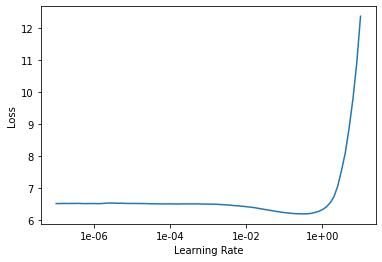
\includegraphics[width=0.465\linewidth]{plots/lm1}
		\label{fig:lm1}
	}
	\subfigure[LR for Target Task]
	{
		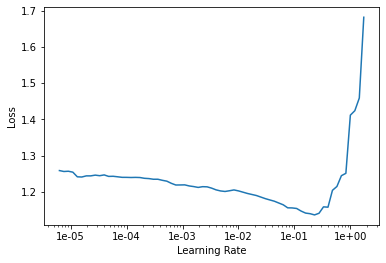
\includegraphics[width=0.465\linewidth]{plots/lm2}
		\label{fig:lm2}
	}
	\caption{Determining Learning Rate}
	\label{fig:lr}
\end{figure}



  
To train the language model during fine-tuning, we chose to unfreeze all the layers and then perform training for 5 epochs due to our computational constraints. The gradual unfreezing helps in avoiding ``catastrophic forgetting'', as explained in \cite{howard2018universal}. This step took significantly more time (1 hour in our case using Tesla K80 GPUs). After fine-tuning, we saved the encoder and the vocabulary 
%(in a pickle file) 
for future use. 
\begin{table}[h!]
	\centering
	\resizebox{0.35\textwidth}{!}{%
		\begin{tabular}{@{}rrrrr@{}}
			\toprule
			\multicolumn{1}{l}{\textbf{epoch}} & \multicolumn{1}{l}{\textbf{train\_loss}} & \multicolumn{1}{l}{\textbf{valid\_loss}} & \multicolumn{1}{l}{\textbf{accuracy}} & \multicolumn{1}{l}{\textbf{time}} \\ \midrule
			0                                  & 4.592715                                 & 4.344318                                 & 0.250712                              & 10:37                             \\
			1                                  & 4.383563                                 & 4.187261                                 & 0.265000                              & 10:37                             \\
			2                                  & 4.192356                                 & 4.110231                                 & 0.270790                              & 10:38                             \\
			3                                  & 4.029832                                 & 4.088607                                 & 0.274656                              & 10:38                             \\
			4                                  & 3.928093                                 & 4.095024                                 & 0.274406                              & 10:37                             \\ \bottomrule
		\end{tabular}%
	}
\caption{Unfreezing the entire model}
\end{table}


%Now as our LM is fine-tuned according to target language distribution, 
Next, we fine-tuned our classifier for stance detection which was our target task.
%We split our data set (of 6.8k tweets) into training and validation set of 80\% and 20\% respectively. 
Just as before to find out the optimum learning rate for our classifier, we plot the learning rate curve in Figure \ref{fig:lm2}. A quick inspection of plot tells us that optimal learning rate should be between $1\times 10^{-3}$ and $1\times 10^{-4}$. We chose $1\times 10^{-3}$, beyond which the loss diverges. While training, we chose to gradually unfreeze our layers. 




Testing our classifier on validation set has produced good results, same is shown in Table \ref{tab:res2} under column name (ULMFiT+AV : where AV stands for Augmented Vocabulary). 